\documentclass[10pt,twocolumn]{article}
\usepackage[margin=0.75in]{geometry}
\usepackage{amsmath,amssymb,booktabs,graphicx,microtype,xcolor,url}
\usepackage[font=small,labelfont=bf]{caption}
\usepackage[numbers,sort&compress]{natbib}
\usepackage[colorlinks=true,linkcolor=blue!50!black,citecolor=blue!50!black,urlcolor=blue!50!black]{hyperref}
\graphicspath{{../results/}{../results/figures/}}
\newcommand{\todo}[1]{\textcolor{red!70!black}{[#1]}}
\newcommand{\E}{\mathbb{E}}
\setlength{\parskip}{2pt}

\title{Foresight: Latency-Aware Anticipatory Bracing for Humanoids\\from Depth Perception}
\author{Prasuna Chatla\\ Stanford University, AA228/CS238 (Autumn 2026) \\ \texttt{pchatla@stanford.edu}}
\date{}

\begin{document}
\maketitle

\begin{abstract}
A walking humanoid that sees an object approaching through delayed, noisy and intermittent detections must decide whether to keep walking and rely on reactive balance, or to interrupt locomotion and brace: a posture that absorbs a larger impulse at contact but costs progress, must be held for a minimum commitment, and is wasted if the object misses. We pose this as a POMDP over two frozen reinforcement-learned skills on a Unitree G1 in MuJoCo Playground, with the object's mass unobservable, and build every layer of the pipeline in simulation: an impact environment with paired, replayable disturbances; a BRACE skill trained to take over from walking states; a Rao-Blackwellized belief over the object; and decision rules compared on a failure-rate versus false-preparation frontier against a privileged oracle. We find that (i) preparation is worth having: with privileged timing, bracing cuts the failure rate on identical impacts from 0.70 to 0.42, while merely stopping does nothing; (ii) a belief-based commit rule is the most selective decision method but, at 10\,Hz detections, cannot reach the failure rate of a time-to-contact threshold; (iii) raising the detection rate to 50\,Hz does not close the gap, because the limiting factor is not when the belief resolves (0.46\,s before contact at 50\,Hz) but a release defect in the rule's commitment logic, which a calibration study exposed; and (iv) a geometric detector on rendered depth measures a 3\,cm, range-independent noise, a 94\% detection rate and a 90$^\circ$ usable field of view, replacing the assumed observation model. \todo{Session E: corrected rule, oracle-gap ladder, ablations, object-aware PPO baseline.} Code, results and checkpoints: \url{https://github.com/pchatla-arch/anticipatory-balance}.
\end{abstract}

\section{Introduction}
Legged robots recover from pushes reactively: a learned or model-based balance controller responds once the disturbance is felt. A robot that can see the disturbance coming has an option the reactive controller does not: to prepare. Preparation is not free. A braced posture does not walk, it needs time to form, and if the object misses the cost was paid for nothing. The decision of \emph{whether and when} to prepare is therefore sequential and made under uncertainty about the object's path, timing and mass, from observations that arrive late and only sometimes.

This project studies that decision in isolation. The low-level skills (walking, bracing) are fixed reinforcement-learned policies; the object of study is the decision layer that switches between them from a belief, and what limits it. The questions are concrete: Is bracing worth anything at all against the disturbances a walking humanoid cannot absorb? If so, how much lead time does the posture need? Can a belief over the object, with the mass unobservable, deliver a decision that is both early enough and selective enough? And which part of the pipeline, sensing or deciding, is the binding constraint?

Our contributions are an environment and a paired evaluation protocol in which these questions can be answered without confounds; the measured answer to each of them; and a negative result turned into a diagnosis: the belief rule's shortfall is not a sensing-rate problem, as the first results suggested, but a commitment-logic defect found through a calibration study. \todo{Finish with the corrected rule's result.}

\section{Related work}
Push recovery for humanoids is classically analysed with the linear inverted pendulum and the capture point \citep{pratt2006capture,koolen2012capturability}: the zero-step capturable region gives the impulse a fixed support can absorb, and stepping extends it. We use the zero-step budget as an analytical reference, not as a controller. Learned locomotion policies trained with domain randomization and random pushes \citep{zakka2025playground} recover from moderate disturbances reactively; our walker is Playground's G1 joystick policy trained in our impact environment. Sequential decision making under partial observability is the POMDP framework \citep{kaelbling1998pomdp,kochenderfer2022algorithms}; QMDP \citep{littman1995qmdp} and myopic value-of-information rules are the standard approximations when the belief is tractable but the full problem is not. Anticipatory behaviour in robots, such as pre-impact posture selection for falls \citep{kajita2010fall}, chooses an action once a fall is certain; our setting is the decision before certainty, with a commitment cost.

\section{Problem}
\paragraph{Setting.} A Unitree G1 walks at a commanded forward velocity (0.5\,m/s). A rigid sphere (radius 0.15\,m, mass $m\in[4,16]$\,kg, speed $v\in[3,8]$\,m/s) is launched from 3--5\,m, from an azimuth within $\pm60^\circ$ of the heading, on a straight gravity-compensated path aimed at the pelvis led by the base velocity, arriving 1.5--3.5\,s into the episode. With probability 0.3 the path is offset laterally by 0.4--0.8\,m (a near-miss). Contact is detected by sensors on the torso, pelvis and thighs; failure is the walker's termination condition or sustained tilt.

\paragraph{Actions and skills.} At 10\,Hz the decision layer chooses CONTINUE or BRACE. CONTINUE runs the frozen walker. BRACE zeroes the velocity command and runs a second frozen policy trained to stand low and wide with both feet planted; once started it is held for a minimum commitment $\tau_{\text{commit}}=0.3$\,s. The posture needs $\tau_{\text{brace}}$ to form, a quantity we measure.

\paragraph{POMDP.} Hidden state: the robot's balance state, active skill and remaining commitment, and the object's position, velocity and mass. Observations: detections of the object's position with capture timestamps, delivered every $T_{\text{det}}$ with latency $\ell$, range-dependent noise, a field of view and random misses, or nothing. Reward per interval: $-c_{\text{track}}$ for lost tracking and $-c_{\text{prep}}$ while braced; a one-time $-c_{\text{fall}}$ on failure. We report the two components separately, as the failure rate on scheduled hits and the false-preparation rate on near-misses (plus forward progress), because the cost ratio is a design choice and a frontier shows every choice at once.

\section{Method}
\paragraph{Skills.} The walker is Playground's G1 joystick PPO policy \citep{zakka2025playground} trained in the impact environment with projectiles present (200M steps, 4096 environments, about 20\,min on an RTX~6000~Ada; three seeds, evaluation reward 7.32--7.62). BRACE~v1 was trained from standing resets. BRACE~v2 was trained with the frozen walker in control for the first 0--2\,s of every episode and impacts present afterwards, so that it learns to take over from walking states; its reward is Playground's stand-still tracking with a lower base-height target (0.65\,m), a wider stance target (0.35\,m) and a both-feet-down term.

\paragraph{Paired evaluation.} All comparisons share reset keys and replay the same world-space projectile trajectory (launch position and velocity recorded from a CONTINUE reference rollout), so that every condition meets the same object. Without this, a policy that stops walking also leaves the aim point, and ``dodging by stopping'' masquerades as recovery. No-projectile controls isolate the cost of switching; a zero-command walker isolates stopping from the posture. The actor's command observation is made consistent with its mode in the step it is chosen.

\paragraph{Perception.} A parametric detector delivers the object's world position every $T_{\text{det}}$ steps, captured $\ell$ steps earlier, with noise $\sigma_0+\sigma_1 r$, a 120$^\circ$ field of view and a 5\% miss probability; these numbers are then measured from rendered depth (Section~\ref{sec:e8}).

\paragraph{Belief.} The flight is straight and unaccelerated, so the position--velocity part of the belief is exactly Gaussian and a Kalman filter is exact. A detection captured $\ell$ steps ago is a \emph{linear} measurement of the current state, $z = p_t - \ell\,\Delta t\, v_t + \epsilon$, so a late detection is absorbed exactly without storing past beliefs. The mass is unobservable from position tracks and is carried as samples from the prior. Belief statistics (hit probability $p$, expected time to contact $\E_b[t_{\text{hit}}]$, expected momentum) are Monte-Carlo over the Gaussian and the mass samples, in the robot's frame of commanded motion, with a decision radius $r_c=0.45$\,m about the pelvis axis.

\paragraph{Decision rules.} \emph{Reactive} never braces. \emph{Always} braces when $p>0.3$. \emph{Threshold} braces when the point estimate predicts a hit within $\theta$ seconds. The \emph{belief commit rule} braces when
\begin{equation}
\begin{aligned}
p\,\E_b[\Delta P(J)]\,c_{\text{fall}} &> c_{\text{prep}}\,(\E_b[t_{\text{hit}}]+h) + c_{\text{track}}\,\E_b[t_{\text{hit}}]\\
\text{and}\quad \E_b[t_{\text{hit}}] &> \tau_{\text{brace}},
\end{aligned}
\label{eq:rule}
\end{equation}
where $\Delta P(J)=P(\text{fall}\mid\text{CONTINUE},J)-P(\text{fall}\mid\text{BRACE},J)$ is a logistic response model in $\log J$ fitted on the oracle data (Section~\ref{sec:gate}) and averaged over the mass mixture through $J=m|v|$. Read: brace when the expected failure risk removed outweighs the cost of being braced until the impact (plus a hold $h$), and only if the posture still has time to form. The \emph{oracle} switches at a fixed lead before the true arrival. All rules share the commitment and release logic.

\paragraph{Analytical reference.} For standing contacts, the zero-step capture-point budget $J_{\max}=m_r\,\omega\,(x_{\text{edge}}-x_{\text{cp}})$ with $\omega=\sqrt{g/z}$ and $x_{\text{cp}}=x+\dot x/\omega$ from the measured CoM and feet is compared with the incoming momentum.

\section{Experiments}
\subsection{Disturbance regime and the capture-point reference}
On the originally proposed range (1--8\,kg, 1--4\,m/s) the walker failed in 0.46\% of 4,096 scheduled hits, and only 31\% made contact, so that range does not test anticipation. Extending to 4--32\,kg and 2--8\,m/s gives a graded failure surface (Fig.~\ref{fig:surfaces}). Equal incoming momentum is not equal severity: at 32\,N\,s, 4\,kg at 8\,m/s fails 92\% of standing trials, 8\,kg at 4\,m/s 48\%, 16\,kg at 2\,m/s 9\%. The zero-step budget (median 13.1\,N\,s at a 0.671\,m CoM) agrees with the recorded outcome on 73.6\% of 2,041 standing contacts (always-fail baseline 64.9\%), catching 1,320 of 1,325 failures but flagging 534 of 716 survivors: a screening feature with high sensitivity, not a bound (Fig.~\ref{fig:lip}). During walking the capture point lies outside the support polygon by construction and the fixed-support calculation does not apply (accuracy 53\%). The decision experiments use the regime where the walker, walking, fails 70\% of the time given contact: 4--16\,kg at 3--8\,m/s with the led aim, contact 98--100\%.

\begin{figure}[t]\centering
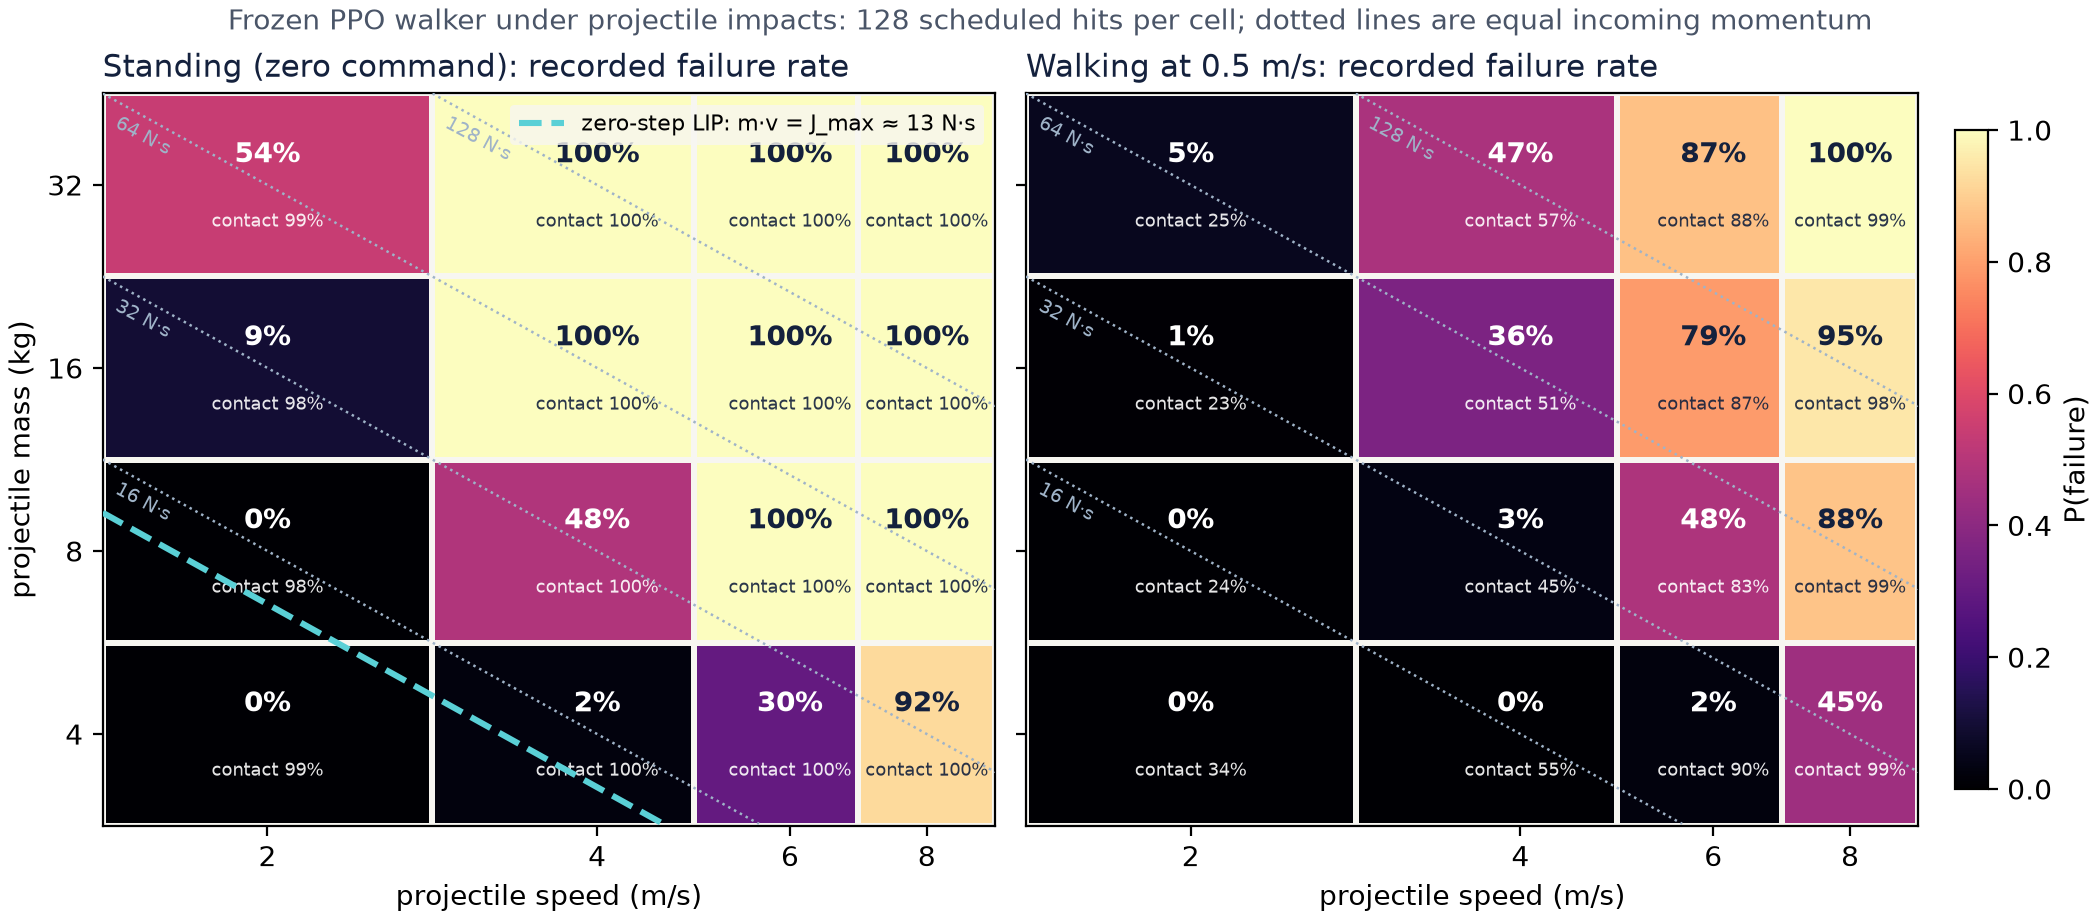
\includegraphics[width=\linewidth]{fall_surfaces.png}
\caption{Recorded failure rate of the frozen walker, standing (left) and walking (right), 128 scheduled hits per cell with the contact rate in each cell. Dotted lines: equal incoming momentum; dashed: the zero-step capture-point reference.}\label{fig:surfaces}
\end{figure}
\begin{figure}[t]\centering
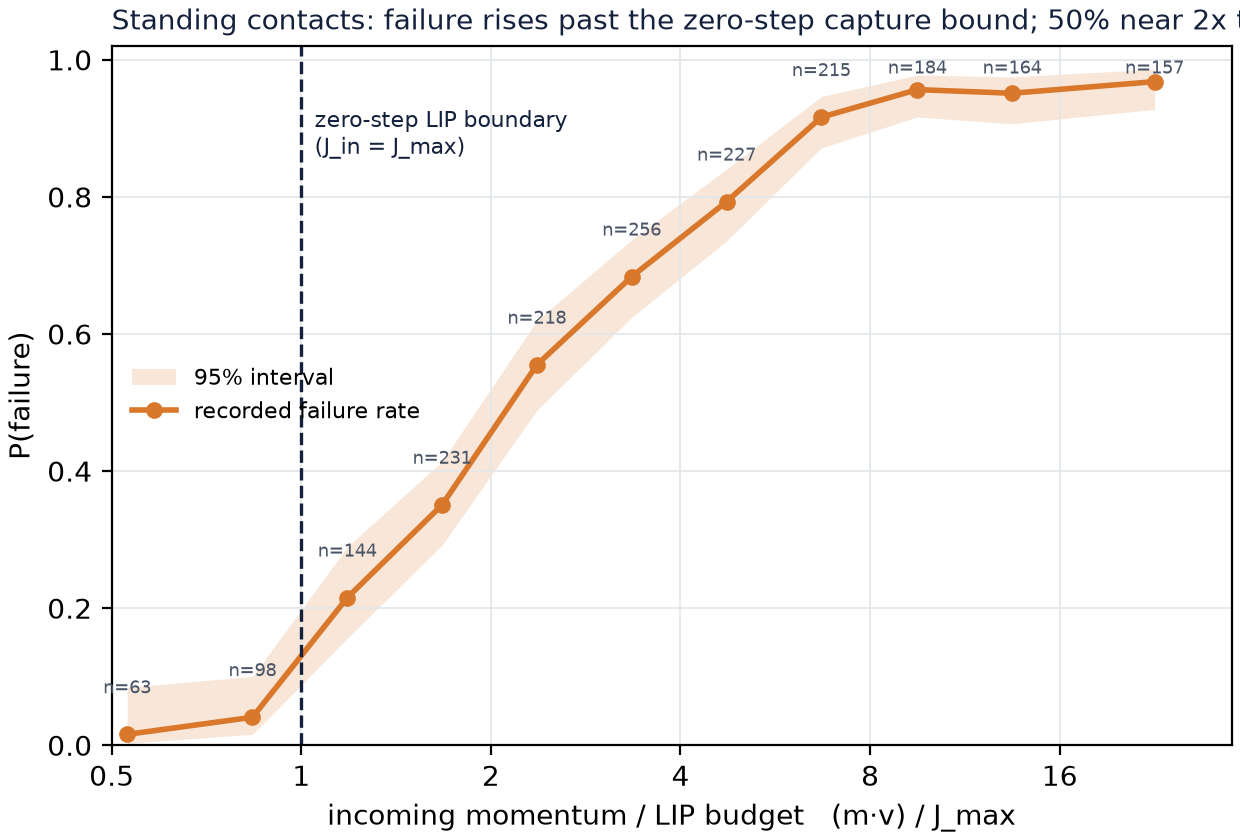
\includegraphics[width=0.8\linewidth]{lip_ratio_curve.png}
\caption{Standing contacts binned by incoming momentum over the zero-step budget (Wilson 95\% intervals). Failure is 21\% just past the boundary and 50\% near twice the budget.}\label{fig:lip}
\end{figure}

\subsection{Is bracing worth anything? The evidence gate}\label{sec:gate}
A privileged rule switched from the walker to BRACE at several leads before the nominal arrival, on 512 paired scenarios per condition. The first attempt, with BRACE~v1 and the uncorrected evaluator, raised the failure rate from 0.2\% to 38--74\%, rising with lead, and at 0.5\,s lead 270 of 337 failures occurred with no contact at all. No-projectile controls then showed that switching to either BRACE policy fails only 0--3\%: the failures were the evaluator's one-step lag between the switch and the command observation, not the skill. With the corrected protocol and BRACE~v2 (Table~\ref{tab:gate}), failure given contact falls from 0.70 to 0.42 at 0.5\,s lead on identical impacts, while a zero-command walker stays at 0.69--0.70. Stopping does nothing; the posture protects, once it has had time to form. The sustained readiness criterion (pelvis within 3\,cm of its target height, torso upright, both feet down for 0.2\,s) is met 0.21--0.22\,s after the switch, which fixes $\tau_{\text{brace}}=0.22$\,s. Preparation costs 0.49\,m of the 2.55\,m the walker covers in an episode when the object misses. At leads of 0.75\,s or more the braced robot is no longer where the replayed trajectory was aimed (contact 80\% and 40\%); those rows are reported but not used, and the oracle lead is fixed at 0.5\,s.

\begin{table}[t]\centering\small
\caption{Oracle test with BRACE~v2 on shared replayed impacts (4--16\,kg, 3--8\,m/s, 512 scenarios per cell). Failure given contact; the last column is the fraction of episodes in which the posture was ready at impact.}\label{tab:gate}
\begin{tabular}{lcccc}\toprule
Lead (s) & CONTINUE & zero-cmd & BRACE v2 & ready \\\midrule
0.1 & 0.70 & 0.70 & 0.64 & 4\% \\
0.2 & 0.70 & 0.70 & 0.60 & 5\% \\
0.3 & 0.70 & 0.70 & 0.50 & 12\% \\
0.5 & 0.70 & 0.69 & 0.42 & 96\% \\\bottomrule
\end{tabular}
\end{table}

\subsection{Observation model from rendered depth}\label{sec:e8}
The MJX-Warp batch ray-tracer renders the head camera (90$^\circ$ vertical field of view, 96$\times$96) for 128 environments in 40\,ms per batch inside the walking loop (1,000 environment steps per second with a frame every two steps). A geometric detector with no learning and no object model back-projects every valid depth pixel with the camera pose, keeps points above the ground, away from the robot's own body and within range, takes their median and adds one radius along the view ray. Against the true object position over 12,800 frames: a 94.5\% detection rate when the object is in the image, a 5.0\% false-alarm rate, and a per-axis RMS error of 2--3\,cm from 1 to 6\,m with no measurable range dependence (the fit gives $\sigma_0=0.030$\,m, $\sigma_1\approx0$; the assumed model was $0.03+0.02r$), because depth in simulation is exact and the error is pixel quantization. The important correction is the field of view: with launches within $\pm60^\circ$ of the heading, 66\% of frames with a launched object have it outside the 90$^\circ$ image, against the 120$^\circ$ assumed (Fig.~\ref{fig:e8}). \todo{Session E uses the measured values.}

\begin{figure}[t]\centering
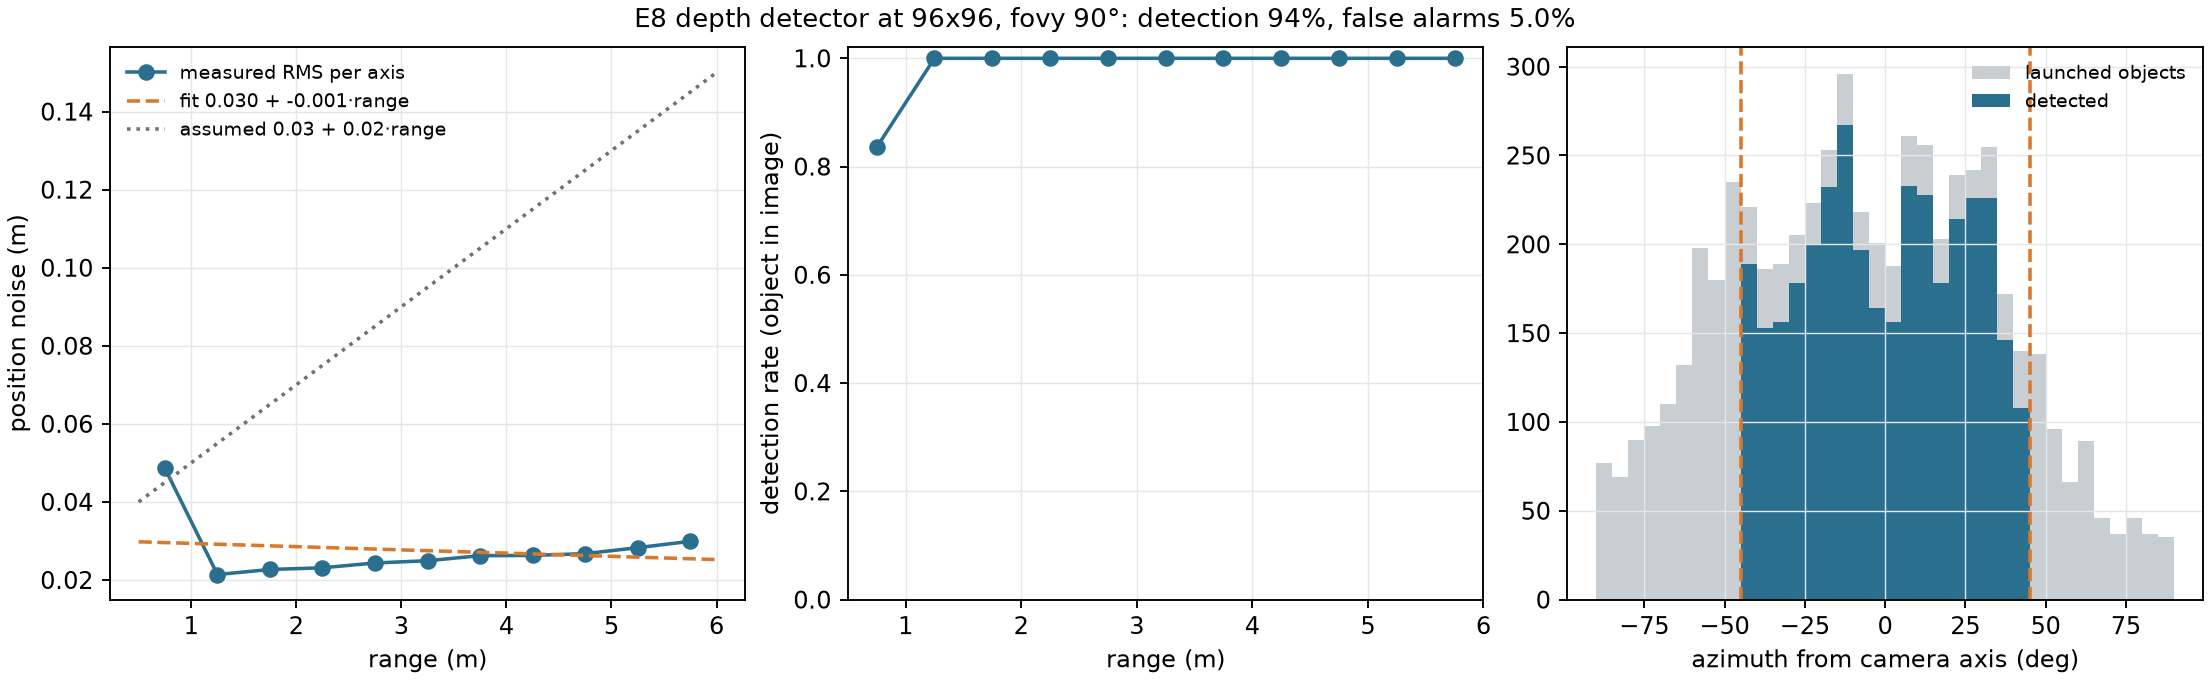
\includegraphics[width=\linewidth]{E8_depth_detector/detector.png}
\caption{Depth detector on rendered frames: noise against range with the assumed model (left), detection rate against range (centre), azimuth of launched objects and of detections with the camera's field of view (right).}\label{fig:e8}
\end{figure}

\subsection{The decision frontier at 10\,Hz}
Reactive, always, the threshold rule ($\theta=0.2$--$0.8$\,s), the belief rule ($c_{\text{prep}}/c_{\text{fall}}=0.02$--$0.8$) and the oracle ran on the same 2,048 paired scenarios (70\% hits, 30\% near-misses) at latencies of 0, 100 and 300\,ms with detections at 10\,Hz (Fig.~\ref{fig:frontier}). Reactive fails 0.69, the oracle 0.36. The threshold rule reaches 0.55 at 37--51\% false preparations; the belief rule is the most selective method, 0.60 at 18\% false preparations against the threshold's 0.60 at 26\%, but it never goes lower, and at 300\,ms latency it barely acts. The first reading was that the belief braces too late: with detections every 100\,ms, 100\,ms old, the hit probability resolves 0.2--0.3\,s before contact, when the brace needs 0.22\,s to form. A threshold at $\theta\ge0.6$\,s braces at first sight; early and sloppy beat late and careful.

\begin{figure*}[t]\centering
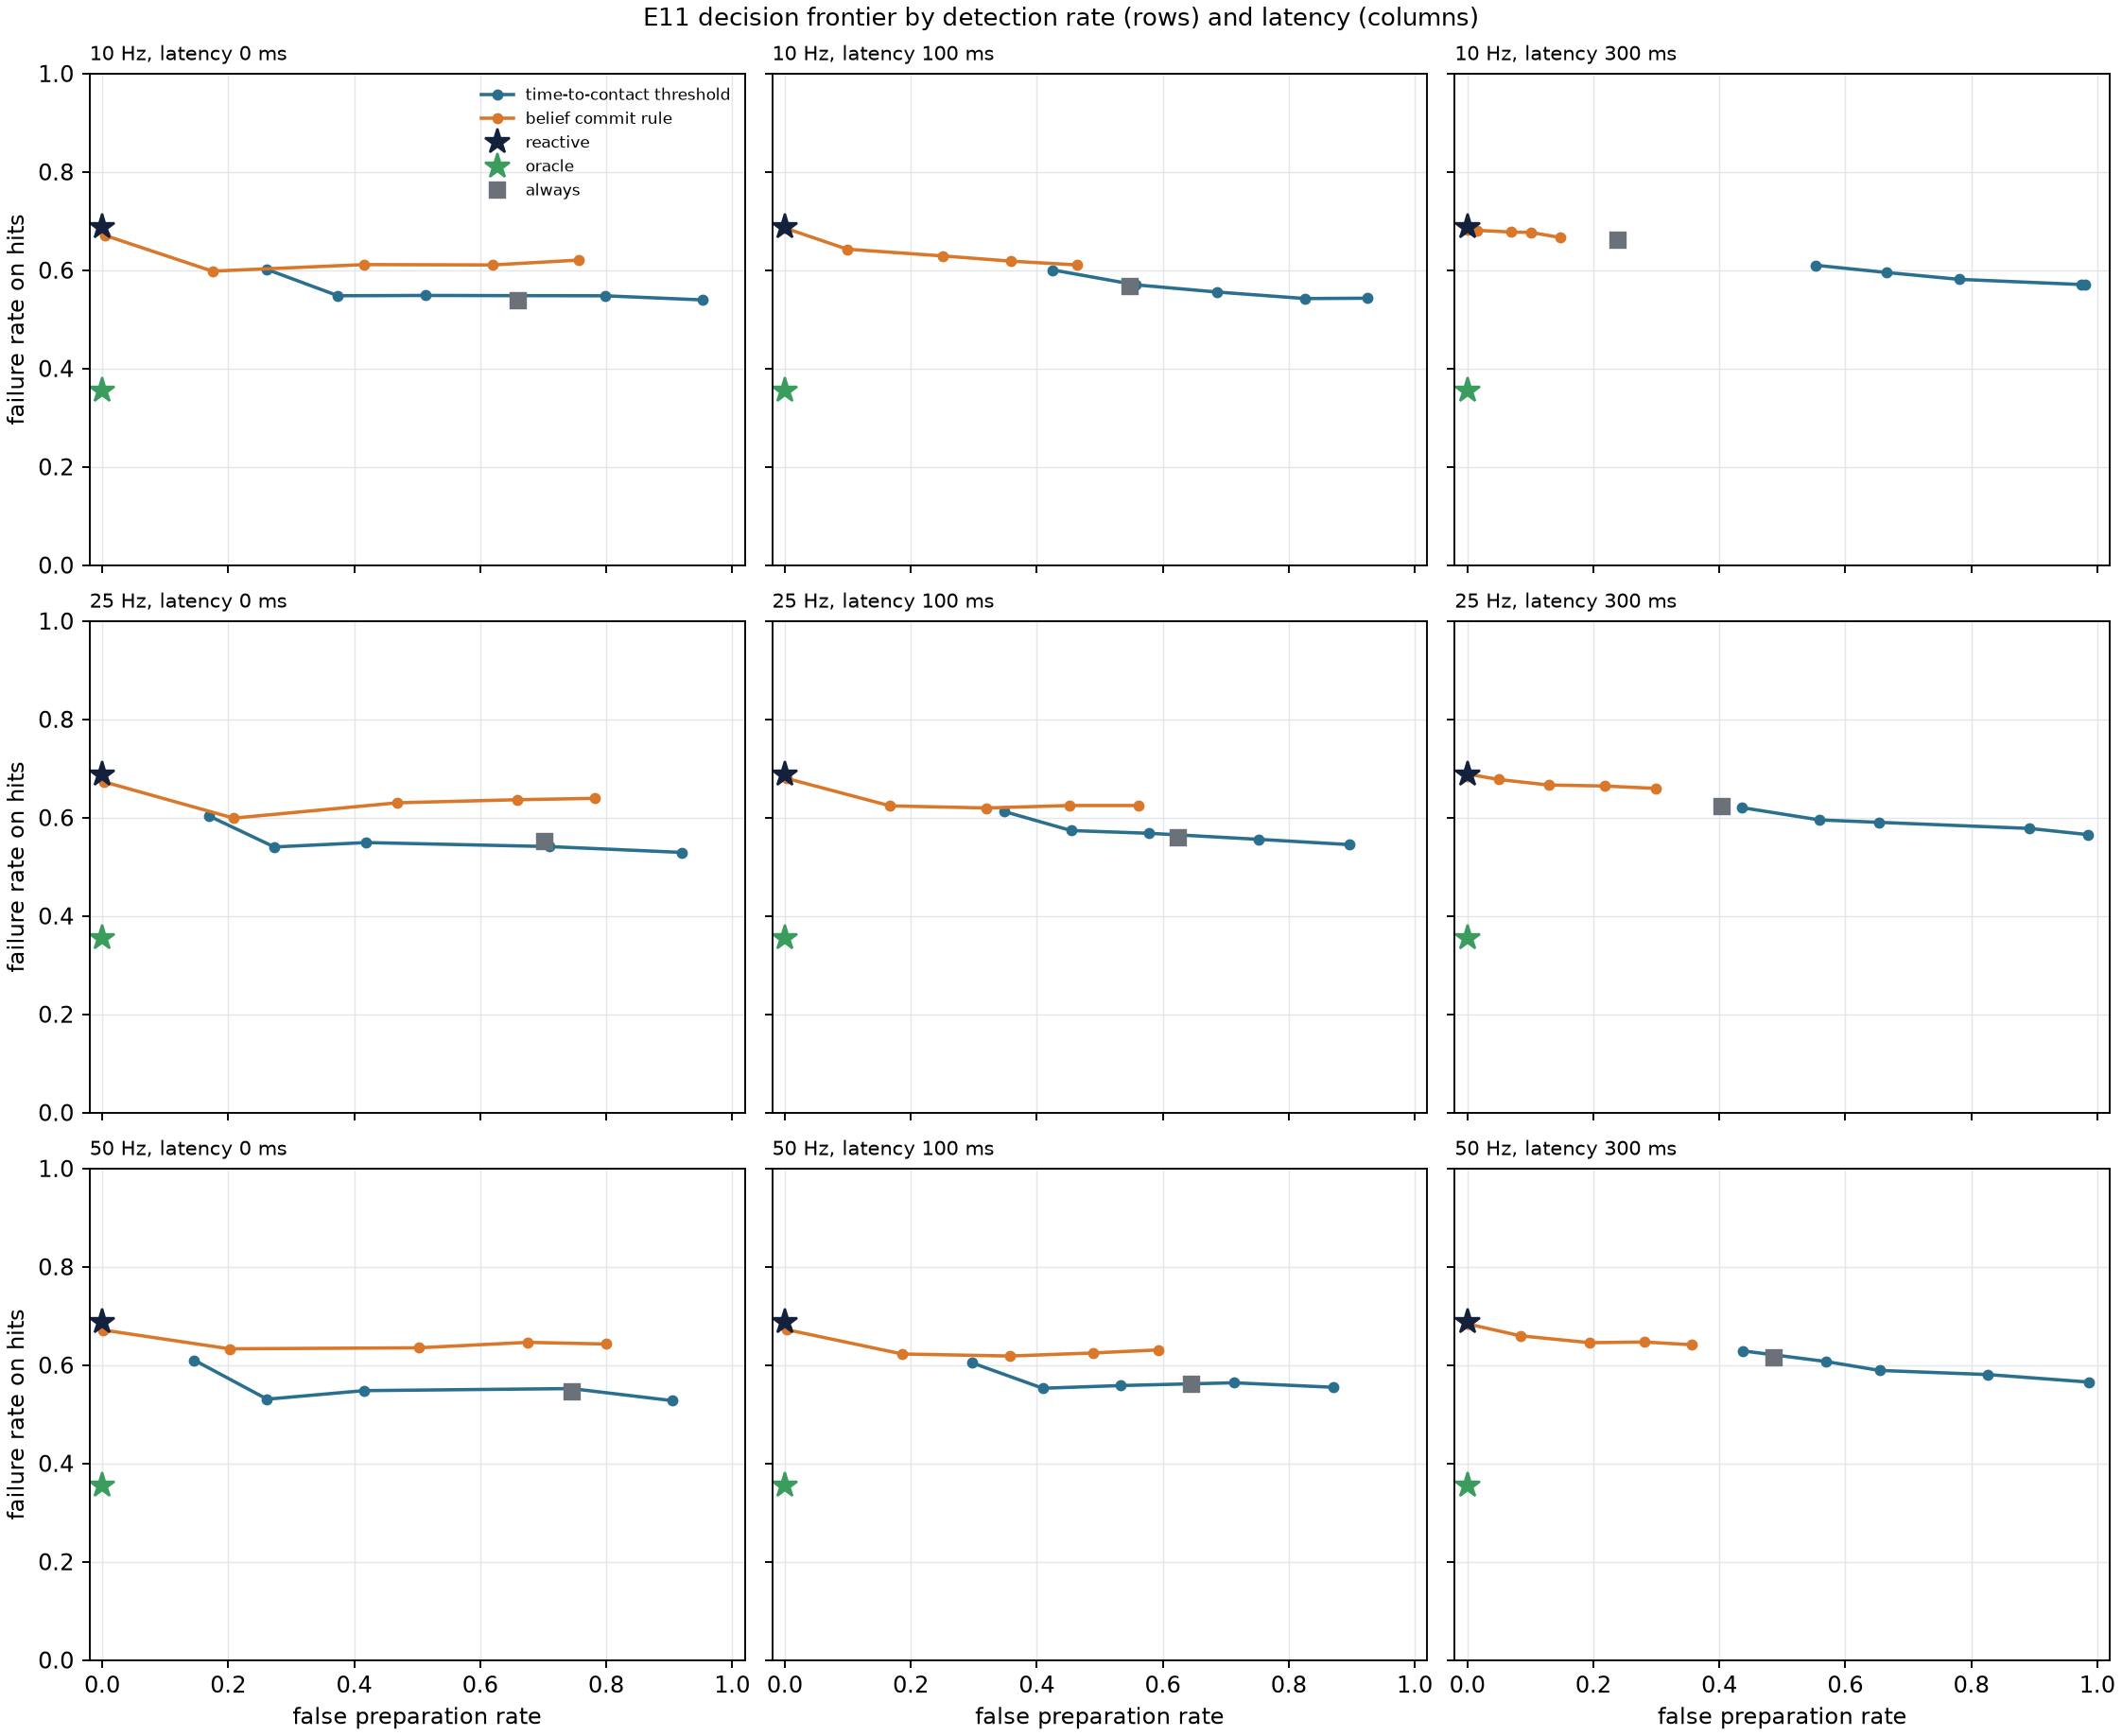
\includegraphics[width=0.95\textwidth]{E11_rate_sweep/frontier_grid.png}
\caption{Decision frontier (failure rate on scheduled hits against false-preparation rate on near-misses; lower-left is better) by detection rate (rows: 10, 25, 50\,Hz) and latency (columns: 0, 100, 300\,ms). Stars: reactive (0.69) and oracle (0.36).}\label{fig:frontier}
\end{figure*}

\subsection{Rate sweep and calibration: the constraint was not sensing}
If the belief were merely late, a higher detection rate should move its curve under the threshold's. It does not (Fig.~\ref{fig:frontier}, Table~\ref{tab:rate}). At 50\,Hz and zero latency the threshold improves slightly (0.53 at 26\% false preparations) and the belief rule gets \emph{worse} (0.63 at 20\%), at every latency. The calibration study (Fig.~\ref{fig:calib}) rules out the belief itself: at 50\,Hz the hit probability is roughly calibrated above $p=0.4$ (expected calibration error 0.18 at zero latency, dominated by the low-$p$ bins where near-misses at 0.4--0.8\,m offset are inside the 0.45\,m decision radius), the time-to-contact estimate is within 0.03\,s of the truth in the last 0.4\,s, and the belief first exceeds $p=0.5$ a median 0.46\,s before contact (interquartile 0.36--0.62\,s), twice $\tau_{\text{brace}}$. The belief resolves in time; the rule still fails.

The per-condition records show why. At low $c_{\text{prep}}$ the belief rule braces on 96--100\% of hits, as often as the threshold, and for longer (0.36\,s against 0.24\,s), yet fails more given contact (0.69 against 0.56). The rule re-evaluated its start condition, Eq.~\eqref{eq:rule}, to decide whether to \emph{stay} braced. The condition contains $\E_b[t_{\text{hit}}]>\tau_{\text{brace}}$; once the belief says contact is less than 0.22\,s away and the 0.3\,s commitment has expired, the rule released the brace and switched back to walking, a mode transition at the worst possible moment. A sharper belief makes the release more precise, which is why more sensing made it worse, and why at 10\,Hz, where the belief resolves late and the commitment still covers the impact, the defect was partly hidden. The corrected rule holds BRACE until the object has passed or the belief has gone stale; the start condition decides only when to start. \todo{E15: corrected-rule frontier at 10 and 50\,Hz; Table~\ref{tab:rate} second block.}

\begin{table}[t]\centering\small
\caption{Best failure rate under a 50\% false-preparation budget, by detection rate and latency (uncorrected rule, Session D). \todo{Add the corrected rule.}}\label{tab:rate}
\begin{tabular}{lcccccc}\toprule
 & \multicolumn{3}{c}{threshold} & \multicolumn{3}{c}{belief rule} \\
latency (ms) & 0 & 100 & 300 & 0 & 100 & 300 \\\midrule
10\,Hz & 0.55 & 0.60 & -- & 0.60 & 0.61 & 0.67 \\
25\,Hz & 0.54 & 0.57 & 0.62 & 0.60 & 0.62 & 0.66 \\
50\,Hz & 0.53 & 0.55 & 0.63 & 0.63 & 0.62 & 0.64 \\\bottomrule
\end{tabular}
\end{table}
\begin{figure}[t]\centering
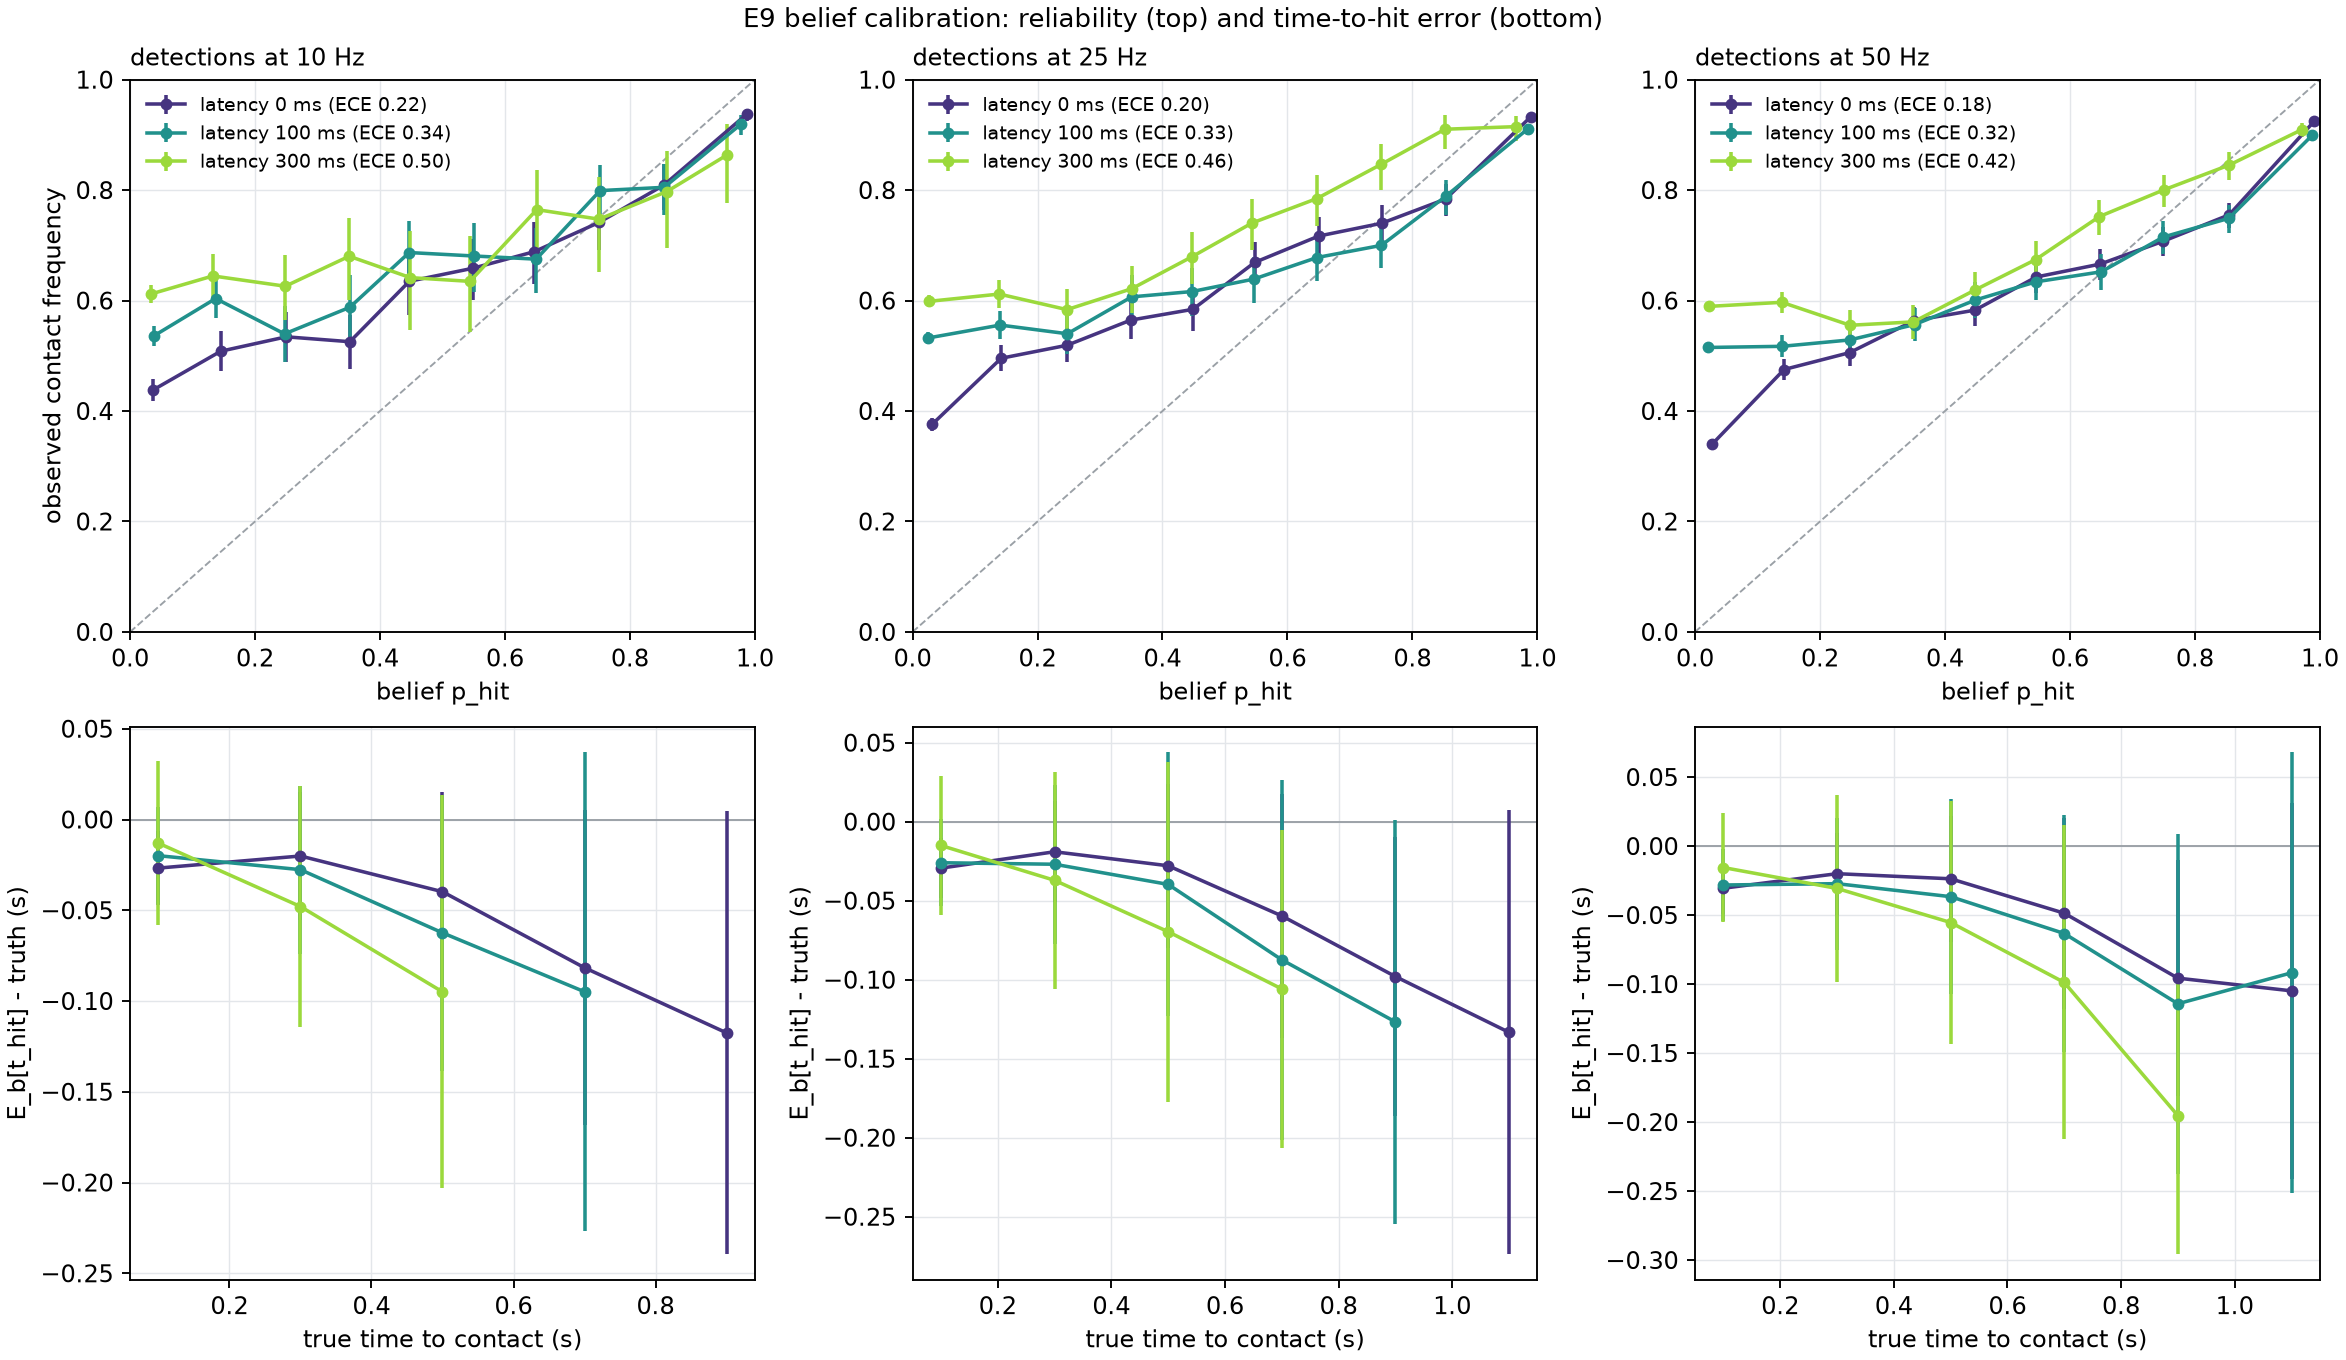
\includegraphics[width=\linewidth]{E9_calibration/calibration.png}
\caption{Belief calibration by detection rate and latency: reliability of the hit probability against the eventual contact (top; Wilson 95\% intervals) and error of the expected time to contact (bottom).}\label{fig:calib}
\end{figure}

\subsection{Oracle-gap ladder, ablations and the end-to-end baseline}
\todo{Session E. E12: reactive $\to$ 10\,Hz $\to$ 50\,Hz $\to$ perfect sensing $\to$ oracle, with the share of the 0.69--0.36 gap each rung removes. E13: commitment 0.1/0.3/0.5\,s, $\tau_{\text{brace}}$ 0.10/0.22/0.35\,s, mass prior true/wide/point, decision radius 0.35\,m, the old release logic. E14: object-aware PPO walker with the same observation model as input, trained with heavy impacts, evaluated on the same scenarios at 10\,Hz/100\,ms and 50\,Hz/0\,ms.}

\section{Discussion and limitations}
\paragraph{What the evidence supports.} Preparation has real value against disturbances the walker cannot absorb (0.70 to 0.42 at identical contact), the value comes from the posture and not from stopping, and the posture needs about 0.22\,s. The belief over a straight-flying object is tractable, exact in its Gaussian part, and resolves early enough at moderate sensing rates. The pipeline's weakest link was the commitment logic, found only because the calibration study separated ``the belief is late'' from ``the belief is wrong'' from ``the rule misuses a good belief''.

\paragraph{What it does not yet support.} Whether a belief-based rule beats a tuned threshold under the corrected logic is the open question for Session E. The mass is unobservable and enters only through the prior; a size-conditioned prior would need varying object sizes. The near-miss offset (0.4--0.8\,m) overlaps the decision radius, so part of the false-preparation rate is the belief correctly flagging objects that pass within half a metre of the pelvis; the ablation at $r_c=0.35$\,m addresses this. The committed skills were trained with the projectile mass randomized over 1--8\,kg (one shared randomizer) and evaluated at 4--16\,kg; BRACE~v2 generalized, but the mismatch is noted and fixed in the code for future training. Results are from one walker seed; the oracle test and the frontier would need repetition across seeds for confidence intervals on the differences between rules. Everything is in simulation with exact depth; a real depth sensor's noise would change $\sigma_0$ and the false-alarm rate, though not the structure of the argument.

\section{Conclusion}
We built and measured every layer of an anticipatory-bracing pipeline for a walking humanoid and used paired, replayable disturbances to ask whether, when and from what a humanoid should brace. Bracing is worth 0.28 in failure rate with privileged timing; a belief that resolves 0.46\,s ahead is available at 50\,Hz; and the decision layer's shortfall traced to a release defect rather than to perception. \todo{Final sentence from Session E.}

\bibliographystyle{plainnat}
\begin{thebibliography}{9}\small
\bibitem[Pratt et al.(2006)]{pratt2006capture} J.~Pratt, J.~Carff, S.~Drakunov, and A.~Goswami. Capture point: a step toward humanoid push recovery. \emph{IEEE-RAS Humanoids}, 2006.
\bibitem[Koolen et al.(2012)]{koolen2012capturability} T.~Koolen, T.~de~Boer, J.~Rebula, A.~Goswami, and J.~Pratt. Capturability-based analysis and control of legged locomotion, part 1. \emph{IJRR}, 31(9), 2012.
\bibitem[Zakka et al.(2025)]{zakka2025playground} K.~Zakka et al. MuJoCo Playground. \emph{arXiv:2502.08844}, 2025.
\bibitem[Kaelbling et al.(1998)]{kaelbling1998pomdp} L.~P. Kaelbling, M.~L. Littman, and A.~R. Cassandra. Planning and acting in partially observable stochastic domains. \emph{Artificial Intelligence}, 101, 1998.
\bibitem[Kochenderfer et al.(2022)]{kochenderfer2022algorithms} M.~J. Kochenderfer, T.~A. Wheeler, and K.~H. Wray. \emph{Algorithms for Decision Making}. MIT Press, 2022.
\bibitem[Littman et al.(1995)]{littman1995qmdp} M.~L. Littman, A.~R. Cassandra, and L.~P. Kaelbling. Learning policies for partially observable environments: scaling up. \emph{ICML}, 1995.
\bibitem[Kajita et al.(2010)]{kajita2010fall} S.~Kajita et al. Falling motion control for humanoid robots. \emph{IEEE-RAS Humanoids}, 2010. \todo{verify citation}
\end{thebibliography}
\end{document}
